% Figure from MATH 591 notes, section 58. Compile with the notes preamble.
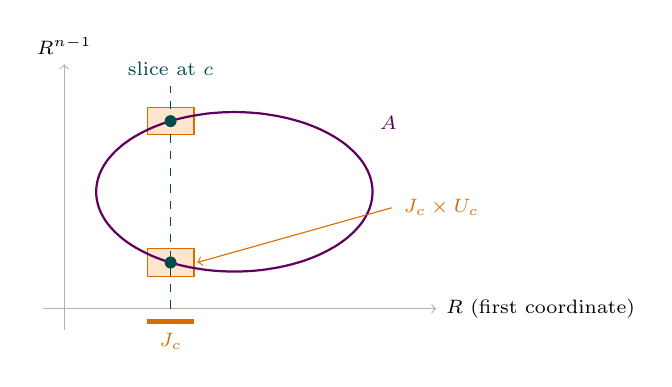
\begin{tikzpicture}[scale=1.35]
\draw[->, gray!60] (-0.2,0) -- (3.5,0) node[right, font=\scriptsize, text=black] {$\mathbb{R}$ (first coordinate)};
\draw[->, gray!60] (0,-0.2) -- (0,2.3) node[above, font=\scriptsize, text=black] {$\mathbb{R}^{n-1}$};
\draw[orange!85!black, fill=orange!20] (0.78,0.305) rectangle (1.22,0.565);
\draw[orange!85!black, fill=orange!20] (0.78,1.635) rectangle (1.22,1.895);
\draw[violet!75!black, thick] plot[smooth] coordinates {(2.9,1.1) (2.898,1.139) (2.893,1.178) (2.884,1.217) (2.872,1.256) (2.856,1.294) (2.836,1.332) (2.814,1.369) (2.788,1.405) (2.758,1.44) (2.726,1.475) (2.69,1.508) (2.652,1.541) (2.61,1.572) (2.566,1.602) (2.519,1.63) (2.47,1.657) (2.418,1.683) (2.364,1.707) (2.308,1.729) (2.25,1.75) (2.19,1.768) (2.129,1.785) (2.066,1.8) (2.002,1.813) (1.936,1.824) (1.87,1.834) (1.803,1.841) (1.736,1.846) (1.668,1.849) (1.6,1.85) (1.532,1.849) (1.464,1.846) (1.397,1.841) (1.33,1.834) (1.264,1.824) (1.198,1.813) (1.134,1.8) (1.071,1.785) (1.01,1.768) (0.95,1.75) (0.892,1.729) (0.836,1.707) (0.782,1.683) (0.73,1.657) (0.681,1.63) (0.634,1.602) (0.59,1.572) (0.548,1.541) (0.51,1.508) (0.474,1.475) (0.442,1.44) (0.412,1.405) (0.386,1.369) (0.364,1.332) (0.344,1.294) (0.328,1.256) (0.316,1.217) (0.307,1.178) (0.302,1.139) (0.3,1.1) (0.302,1.061) (0.307,1.022) (0.316,0.983) (0.328,0.944) (0.344,0.906) (0.364,0.868) (0.386,0.831) (0.412,0.795) (0.442,0.76) (0.474,0.725) (0.51,0.692) (0.548,0.659) (0.59,0.628) (0.634,0.598) (0.681,0.57) (0.73,0.543) (0.782,0.517) (0.836,0.493) (0.892,0.471) (0.95,0.45) (1.01,0.432) (1.071,0.415) (1.134,0.4) (1.198,0.387) (1.264,0.376) (1.33,0.366) (1.397,0.359) (1.464,0.354) (1.532,0.351) (1.6,0.35) (1.668,0.351) (1.736,0.354) (1.803,0.359) (1.87,0.366) (1.936,0.376) (2.002,0.387) (2.066,0.4) (2.129,0.415) (2.19,0.432) (2.25,0.45) (2.308,0.471) (2.364,0.493) (2.418,0.517) (2.47,0.543) (2.519,0.57) (2.566,0.598) (2.61,0.628) (2.652,0.659) (2.69,0.692) (2.726,0.725) (2.758,0.76) (2.788,0.795) (2.814,0.831) (2.836,0.868) (2.856,0.906) (2.872,0.944) (2.884,0.983) (2.893,1.022) (2.898,1.061) (2.9,1.1)};
\draw[teal!60!black, dashed] (1,0) -- (1,2.1) node[above, font=\scriptsize] {slice at $c$};
\fill[teal!60!black] (1,0.435) circle (1.6pt); \fill[teal!60!black] (1,1.765) circle (1.6pt);
\draw[orange!85!black, line width=2pt] (0.78,-0.12) -- (1.22,-0.12) node[below, midway, font=\scriptsize] {$J_c$};
\node[violet!75!black, font=\scriptsize] at (3.05,1.75) {$A$};
\node[orange!85!black, font=\scriptsize, anchor=west] at (3.1,0.95) {$J_c \times U_c$};
\draw[orange!85!black, ->] (3.08,0.95) -- (1.25,0.435);
\end{tikzpicture}
